\makechapteropener
	{三} 
	{不等式}
	{给我五个系数,我将画出一头大象;给我六个,我能让它的鼻子摇晃。} 
	{奥古斯丁·路易·柯西 (Augustin-Louis Cauchy)}
	
	\chapter{不等式}
	
	\lettrine{本}{章我们}将从最基础也最重要的一条不等式——基本不等式(均值不等式)出发,探索其内涵、证明与应用.我们将见识到著名的“调几代平”不等式链,更重要的是,我们将系统学习在求解最值问题时,那些令人拍案叫绝的“配凑”技巧,并掌握证明不等式的三大基本法门.攻克本章,你将获得解决优化问题的利器.
	
	% --- 章节摘要 ---
\begin{introduction}[知识概括]
	\item \textbf{均值不等式:} 深刻理解“一正、二定、三相等”的七字箴言,这是使用均值不等式求最值的大前提.本章的核心计算技巧均围绕“构造定值”这一目标展开.
	\item \textbf{不等式链:} 掌握“平方平均数 $\ge$ 算术平均数 $\ge$ 几何平均数 $\ge$ 调和平均数”这一重要结论,并理解其推导过程,它是不等式体系的延伸和完善.
	\item \textbf{配凑技巧:} 这是本章的灵魂.必须熟练掌握“拆项与凑项”、“凑系数”、“乘1代换”、“平方”等高级技巧,将非标准形式转化为可以应用均值不等式的标准形式.
	\item \textbf{证明方法:} 掌握作差法、分析法和综合法.理解分析法“执果索因”的思考路径与综合法“由因导果”的书写格式,是严谨证明不等式题目的关键.
\end{introduction}
	
	\section{均值不等式}
	
	\subsection{基本不等式}
	
	我们从一个简单而深刻的几何事实出发:对于一个长和宽分别为 $a,b$ 的矩形,其面积为 $ab$;而一个边长为 $\frac{a+b}{2}$ 的正方形,其面积为 $(\frac{a+b}{2})^2$.当周长固定时,正方形的面积最大.这一朴素的认知背后,蕴含着数学中最重要的不等式之一.
	
	\begin{theorem}[基本不等式]
		对于任意两个正实数 $a, b$,我们有:
		\begin{equation}
			\frac{a+b}{2} \ge \sqrt{ab}
		\end{equation}
		当且仅当 $a=b$ 时,等号成立.
	\end{theorem}
	
	\begin{proof}[证明]
		由于 $a, b$ 均为正实数,$\sqrt{a}$ 和 $\sqrt{b}$ 均有意义.
		我们知道,任何实数的平方都非负,所以:
		\begin{equation}
			(\sqrt{a} - \sqrt{b})^2 \ge 0
		\end{equation}
		展开得 $a - 2\sqrt{ab} + b \ge 0$,移项得 $a+b \ge 2\sqrt{ab}$.
		两边同时除以 2,即得 $\frac{a+b}{2} \ge \sqrt{ab}$.
		等号成立的条件是 $(\sqrt{a} - \sqrt{b})^2 = 0$,即 $\sqrt{a} = \sqrt{b}$,考虑到 $a, b$ 均为正数,故 $a=b$.
	\end{proof}
	\qed
	
			\begin{note}[七字箴言:一正、二定、三相等]
				使用基本不等式求最值,必须严格满足三个条件,缺一不可:
				\begin{enumerate}
					\item \textbf{一正}:所涉及的各项变量必须是正数.
					\item \textbf{二定}:在求最小值时,各项的和必须为定值;在求最大值时,各项的积必须为定值.
					\item \textbf{三相等}:取得最值的那个点,必须能使得不等式中的各项相等.如果等号永远取不到,那么最值就不是通过基本不等式求出的.
				\end{enumerate}
			\end{note}
			
			\subsection{均值不等式链 (调几代平)}
			
			基本不等式实际上是算术平均数与几何平均数的大小关系.将这个关系扩展,我们得到一条非常优美的不等式链.
			
			\begin{definition}[四种平均数]
				对于两个正数 $a,b$:
				\begin{itemize}
					\item \textbf{调和平均数 (H)}: $H_2 = \frac{2}{\frac{1}{a}+\frac{1}{b}}$
					\item \textbf{几何平均数 (G)}: $G_2 = \sqrt{ab}$
					\item \textbf{算术平均数 (A)}: $A_2 = \frac{a+b}{2}$
					\item \textbf{平方平均数 (Q)}: $Q_2 = \sqrt{\frac{a^2+b^2}{2}}$
				\end{itemize}
			\end{definition}
			
			\begin{theorem}[均值不等式链]
				对于任意两个正实数 $a,b$,有:
				\begin{equation}
					\sqrt{\frac{a^2+b^2}{2}} \ge \frac{a+b}{2} \ge \sqrt{ab} \ge \frac{2}{\frac{1}{a}+\frac{1}{b}}
				\end{equation}
				即 $Q_2 \ge A_2 \ge G_2 \ge H_2$.当且仅当 $a=b$ 时,所有等号同时成立.
			\end{theorem}
			
			\begin{proof}
				我们已经证明了 $A_2 \ge G_2$.
				\begin{itemize}
					\item \textbf{证明 $Q_2 \ge A_2$}:
					作平方差:
					$Q_2^2 - A_2^2 = \frac{a^2+b^2}{2} - (\frac{a+b}{2})^2 = \frac{2(a^2+b^2) - (a^2+2ab+b^2)}{4} = \frac{a^2-2ab+b^2}{4} = \frac{(a-b)^2}{4} \ge 0$.
					因为 $Q_2, A_2$ 均为正,所以 $Q_2 \ge A_2$.当且仅当 $a=b$ 时取等.
					\item \textbf{证明 $G_2 \ge H_2$}:
					由于 $a,b$ 为正数,$\frac{1}{a}, \frac{1}{b}$ 也为正数.对其应用基本不等式:
					$\frac{\frac{1}{a}+\frac{1}{b}}{2} \ge \sqrt{\frac{1}{a} \cdot \frac{1}{b}} = \frac{1}{\sqrt{ab}}$.
					两边取倒数,并乘以 2,由于都是正数,不等号方向改变:
					$\frac{2}{\frac{1}{a}+\frac{1}{b}} \le \sqrt{ab}$.
					即 $H_2 \le G_2$.当且仅当 $\frac{1}{a}=\frac{1}{b}$,即 $a=b$ 时取等.
				\end{itemize}
				综上,不等式链成立.
			\end{proof}
			\qed

\section{不等式的配凑技巧与思想}

\subsection{方法论}

\textbf{【核心思想】}
\textcolor{green!50!black}{所有配凑技巧的出发点和归宿,都是为了同一个目标:\textbf{创造“定值”}.在使用均值不等式时,我们需要“和为定值”或“积为定值”;在使用柯西不等式时,我们需要某些“平方和”为定值.因此,解题的第一步,是敏锐地观察已知条件和所求表达式的结构特征.}
\begin{itemize}
	\item \textbf{看到分式,想到“拆”与“凑”}:尤其是分母是单项或简单多项式时,往往需要通过拆分分子或配凑系数,创造出与分母相乘为定值的项.
	\item \textbf{看到一次式条件,分式和所求}:形如已知 $ax+by=k$,求 $\frac{m}{x}+\frac{n}{y}$,这是“1的代换”的强烈信号.
	\item \textbf{看到二次式,想到配方与柯西}:条件或所求中出现 $x^2+y^2$ 等形式,优先考虑柯西不等式或二次函数配方法.
	\item \textbf{看到不同次的式子,想到齐次化}:当分式中分子分母次数不同,结构复杂时,考虑通过“除法”等手段,将其变为“整式+分式”的齐次结构.
\end{itemize}

\subsection{技巧一:拆项与凑项法(加减常数)}

\textbf{【原理与逻辑】}
这是最基本的配凑法.其原理在于,当我们有两个正变量 $u,v$,直接使用均值不等式要求 $u+v$ 或 $uv$ 是定值.当它们不是定值时,我们就需要主动去改造其中一个变量.例如,对于 $f(x)=g(x)+\frac{k}{h(x)}$,若 $g(x) \cdot \frac{k}{h(x)}$ 不是常数,我们就想办法把 $g(x)$ 变形为 $c \cdot h(x) + \text{常数}$ 的形式,这样 $c \cdot h(x) \cdot \frac{k}{h(x)}$ 就成了常数.

\begin{exercise}[基础]
	已知 $x>2$,求函数 $f(x) = x + \frac{1}{x-2}$ 的最小值.
\end{exercise}
\begin{solution}
	\textcolor{green!50!black}{直接对 $x$ 和 $\frac{1}{x-2}$ 使用均值不等式,其乘积为 $\frac{x}{x-2}$,不是定值.观察到分母是 $x-2$,我们希望分子中也出现一个 $(x-2)$ 项来与之相乘,从而消去变量.}
	将 $x$ 拆分为 $(x-2)+2$.
		$f(x) = (x-2) + \frac{1}{x-2} + 2$
		
		因为 $x>2$,所以 $x-2 > 0$.\textcolor{red}{(“一正”条件满足)}
		对前两项应用均值不等式:
		$(x-2) + \frac{1}{x-2} \ge 2\sqrt{(x-2) \cdot \frac{1}{x-2}} = 2\sqrt{1} = 2$.
		\textcolor{red}{(“二定”条件,积为定值1,已满足)}
		
		所以 $f(x) \ge 2+2=4$.

		当且仅当 $(x-2) = \frac{1}{x-2}$,即 $(x-2)^2=1$,解得 $x-2=1$(因为$x-2>0$),即 $x=3$ 时,等号成立.\textcolor{red}{(“三相等”条件满足)}
	函数的最小值为 $\textcolor{red}{4}$.
\end{solution}
\qed

\subsection{“对勾函数”模型}
形如 $f(x)=x+\frac{a}{x} \ (a>0)$ 的函数被称为“对勾函数”,因其图像形似一个对勾.
\begin{itemize}
	\item \textbf{定义域}: $(-\infty, 0) \cup (0, +\infty)$
	\item \textbf{奇偶性}: 奇函数,图像关于原点对称.
	\item \textbf{单调性}: 在 $(0, \sqrt{a}]$ 上单调递减,在 $[\sqrt{a}, +\infty)$ 上单调递增;在 $(-\infty, -\sqrt{a}]$ 上单调递增,在 $[-\sqrt{a}, 0)$ 上单调递减.
	\item \textbf{最值}: 当 $x>0$ 时,在 $x=\sqrt{a}$ 处取得最小值 $2\sqrt{a}$;当 $x<0$ 时,在 $x=-\sqrt{a}$ 处取得最大值 $-2\sqrt{a}$.
\end{itemize}
\begin{figure}[H]
	\centering
	\begin{tikzpicture}[scale=0.8]
		\draw[->] (-5,0) -- (5,0) node[below] {$x$};
		\draw[->] (0,-5) -- (0,5) node[left] {$y$};
		\draw[blue, thick, smooth] plot[domain=0.5:4] (\x, {\x+4/\x});
		\draw[blue, thick, smooth] plot[domain=-4:-0.5] (\x, {\x+4/\x});
		\node[blue, right] at (4,5) {$y=x+\frac{4}{x}$};
		\fill[red] (2,4) circle (2pt) node[right] {$(2,4)$};
		\fill[red] (-2,-4) circle (2pt) node[left] {$(-2,-4)$};
	\end{tikzpicture}
	\caption{对勾函数图像}
\end{figure}
\textcolor{green!50!black}{理解对勾函数模型,可以帮助我们快速判断形如 $g(x)+k/g(x)$ 的函数的单调性,以及在等号取不到时,确定最值是在端点取到还是不存在.}

\subsection{技巧二:“1”的代换法(乘“1”代换)}

\textcolor{green!50!black}{为什么“1的代换”如此有效?其本质是\textbf{次数的配平}.}
考虑一个典型问题:已知 $x+2y=1$(这是一个\textbf{1次式}),求 $\frac{1}{x}+\frac{1}{y}$(这是一个\textbf{-1次式})的最小值.
如果我们直接将两者相乘:$(\frac{1}{x}+\frac{1}{y})(x+2y)$,展开后得到的项 $1, \frac{2y}{x}, \frac{x}{y}, 2$ 都是\textbf{0次式}!
其中,$1$ 和 $2$ 是常数项(定值),而 $\frac{2y}{x}$ 和 $\frac{x}{y}$ 是互为倒数关系的项,它们的乘积也是定值.
\textcolor{green!50!black}{结论:将一个-1次的表达式乘以一个1次的条件式,可以“配平”次数,将问题转化为处理我们最喜欢的0次式(常数和倒数),这正是均值不等式的最佳用武之地.}

\begin{exercise}
	已知正数 $x,y$ 满足 $x+2y=1$,求 $\frac{1}{x} + \frac{1}{y}$ 的最小值.
\end{exercise}
\begin{solution}
	\textcolor{green!50!black}{这是一个典型的“和为定值,求分式和最值”问题.直接通分或使用均值不等式都会失败.这正是“1的代换”的标志性信号.}
	\begin{enumerate}
		\item \textbf{乘“1”代换}:
		$\frac{1}{x} + \frac{1}{y} = \left( \frac{1}{x} + \frac{1}{y} \right) \cdot 1 = \left( \frac{1}{x} + \frac{1}{y} \right) (x+2y)$
		
		\item \textbf{展开}:
		$= \frac{x}{x} + \frac{2y}{x} + \frac{x}{y} + \frac{2y}{y} = 1 + \frac{2y}{x} + \frac{x}{y} + 2 = 3 + \left( \frac{2y}{x} + \frac{x}{y} \right)$
		
		\item \textbf{使用均值不等式}:
		因为 $x,y$ 为正数, 所以 $\frac{2y}{x} > 0, \frac{x}{y} > 0$.
		对括号内部分使用均值不等式:
		$\frac{2y}{x} + \frac{x}{y} \ge 2\sqrt{\frac{2y}{x} \cdot \frac{x}{y}} = 2\sqrt{2}$
		
		\item \textbf{得出最小值}:
		所以 $\frac{1}{x} + \frac{1}{y} \ge 3 + 2\sqrt{2}$.
		
		\item \textbf{检验等号}:
		当且仅当 $\frac{2y}{x} = \frac{x}{y}$,即 $x^2 = 2y^2$, $x = \sqrt{2}y$ 时取等.
		代入 $x+2y=1$ 中,有 $\sqrt{2}y+2y=1$, 解得 $y = \frac{1}{2+\sqrt{2}}$.存在这样的 $x,y$.
	\end{enumerate}
	$\frac{1}{x} + \frac{1}{y}$ 的最小值为 $\textcolor{red}{3 + 2\sqrt{2}}$.
\end{solution}
\qed

\subsection{技巧三:齐次化(分离常数)}
当遇到形如 $\frac{ax^2+bx+c}{dx+e}$ 的分式,分子分母次数不同,结构不整齐,直接使用任何不等式都很困难.齐次化的思想,是通过\textbf{多项式除法}或类似方法,将其分离成“\textbf{整式 + 真分式}”的结构.这样处理后,往往能转化成我们熟悉的、可以使用拆凑法或均值不等式的形式.

\begin{exercise}
	已知 $x>0$,求 $f(x) = \frac{x^2+2x+5}{x+1}$ 的最小值.
\end{exercise}
\begin{solution}
	\textcolor{green!50!black}{分子是二次,分母是一次,次数不同.我们需要齐次化.方法一是用多项式长除法;方法二是在分子中“配凑”出分母的因式.}
	\begin{enumerate}
		\item \textbf{分子配凑}:
		$f(x) = \frac{x^2+2x+5}{x+1} = \frac{x(x+1)+x+5}{x+1} = x + \frac{x+5}{x+1}$
		\textcolor{green!50!black}{还不够,继续对剩下的分式进行配凑.}
		$f(x) = x + \frac{(x+1)+4}{x+1} = x + 1 + \frac{4}{x+1}$
		
		\item \textbf{转化为拆凑法问题}:
		现在问题变成了求 $(x+1)+\frac{4}{x+1}$ 的最小值.
		令 $t=x+1$,因为 $x>0$,所以 $t>1$.问题是求 $t+\frac{4}{t}$ 在 $t \in (1, \infty)$ 的最小值.
		
		\item \textbf{使用均值不等式}:
		因为 $t>0$, 所以 $t+\frac{4}{t} \ge 2\sqrt{t\cdot\frac{4}{t}} = 4$.
		
		\item \textbf{检验等号}:
		当且仅当 $t = \frac{4}{t}$,即 $t^2=4, t=2$ (因 $t>0$).
		$t=2$ 对应 $x+1=2 \implies x=1$.
		因为 $x=1$ 在定义域 $x>0$ 内,所以等号可取.
	\end{enumerate}
	最小值为 $\textcolor{red}{4}$.
\end{solution}
\qed

\subsection{技巧四:柯西不等式的配凑}

柯西不等式的配凑比均值不等式更灵活.当我们面对的目标函数或约束条件,可以通过“开方”或“平方”凑成柯西不等式的标准形式 $(a^2+b^2)(x^2+y^2) \ge (ax+by)^2$ 时,就可以考虑使用它.

\begin{exercise}
	已知 $x,y$ 均为正数,且 $x+2y=xy$,求 $2x+y$ 的最小值.
\end{exercise}
\begin{solution}
	\textcolor{green!50!black}{这个条件 $x+2y=xy$ 非常不寻常.直接处理很困难.我们可以尝试对它进行变形.两边同除以 $xy$ (因为 $x,y$ 为正数,可以除),看看能得到什么.}
	\begin{enumerate}
		\item \textbf{变形条件}:
		$x+2y=xy \implies \frac{x}{xy} + \frac{2y}{xy} = 1 \implies \frac{1}{y} + \frac{2}{x} = 1$.
		\textcolor{green!50!black}{现在条件变成了一个我们熟悉的“分式和为定值”的形式.}
		
		\item \textbf{构造柯西不等式}:
		我们要求 $2x+y$ 的最小值.
		我们有两个部分:条件 $\frac{2}{x}+\frac{1}{y}=1$ 和目标 $2x+y$.
		考虑使用“1的代换”,但是这次我们用柯西不等式来处理.
		设 $S = 2x+y$.
		$S = S \cdot 1 = (2x+y)(\frac{2}{x}+\frac{1}{y})$.展开后不是很好处理.
		
		\textbf{尝试直接构造柯西不等式:}
		$S = (\sqrt{2x})^2 + (\sqrt{y})^2$.
		条件是 $\frac{2}{x}+\frac{1}{y} = (\frac{\sqrt{2}}{\sqrt{x}})^2 + (\frac{1}{\sqrt{y}})^2 = 1$.
		
		套用柯西不等式 $(a^2+b^2)(x^2+y^2) \ge (ax+by)^2$:
		令 $a=\sqrt{2x}, b=\sqrt{y}$; $x'=\frac{\sqrt{2}}{\sqrt{x}}, y'=\frac{1}{\sqrt{y}}$.
		$(a^2+b^2)(x'^2+y'^2) \ge (ax'+by')^2$
		
		\item \textbf{代入并计算}:
		$(2x+y) \left( \frac{2}{x}+\frac{1}{y} \right) \ge \left( \sqrt{2x}\cdot\frac{\sqrt{2}}{\sqrt{x}} + \sqrt{y}\cdot\frac{1}{\sqrt{y}} \right)^2$
		$(2x+y) \cdot 1 \ge (2+1)^2 = 9$.
		
		\item \textbf{得出最小值}:
		所以 $2x+y \ge 9$.
		
		\item \textbf{检验等号}:
		当且仅当 $\frac{\sqrt{2x}}{\sqrt{2}/\sqrt{x}} = \frac{\sqrt{y}}{1/\sqrt{y}}$.
		$\frac{\sqrt{2x}\sqrt{x}}{\sqrt{2}} = \frac{\sqrt{y}\sqrt{y}}{1} \implies x=y$.
		代入条件 $\frac{2}{x}+\frac{1}{y}=1$ 中:
		$\frac{2}{x}+\frac{1}{x}=1 \implies \frac{3}{x}=1 \implies x=3$.
		所以 $x=y=3$ 时,等号成立.
	\end{enumerate}
	\textbf{【最终答案】} $2x+y$ 的最小值为 $\textcolor{red}{9}$.
\end{solution}
\qed

\section{观察次数大作战}

	欢迎来到“观察次数大作战”!在这里,我们将把“配凑”的艺术提升到一个新的层次.我们不再仅仅是机械地进行拆项、凑系数,而是要学会用一双“火眼金睛”去\textbf{观察代数式中各项的“次数”}.
	\textbf{核心战术思想}:均值不等式的威力,在于它能处理“和”与“积”的关系.而当我们发现,若将若干项相乘,它们的变量可以互相抵消,最终得到一个常数(我们称之为“\textbf{零次式}”)时,均值不等式的大门就向我们敞开了.
	例如,对于 $x$ 和 $\frac{1}{x}$,我们可以非正式地认为它们的次数分别是 \textbf{1次} 和 \textbf{-1次}.它们的乘积 $x \cdot \frac{1}{x} = 1$ 就是一个 \textbf{0次} 的常数.
	本节的挑战,就是训练你通过观察和调整各项的“次数”,使其乘积变为“0次式”,从而克敌制胜!准备好了吗?战斗开始!

% \degree{次数}{表达式}
\newcommand{\degree}[2]{%
	\tikz[baseline=(M.base)] {
		\node[inner sep=0pt] (M) {$#2$}; 
		\node[draw, circle, red, inner sep=1pt, font=\tiny, above=1.5pt] at (M.north) {$#1$}; 
	}%
}

\begin{problemset}
	
	\item \textbf{[第一关]} 已知 $x>0$,求函数 $f(x) = x^2 + \frac{2}{x}$ 的最小值.
	
	\item \textbf{[第二关]} 已知 $x>-2$,求函数 $f(x) = \frac{x^2+5}{x+2}$ 的最小值.
	
	\item \textbf{[第三关]} 已知正数 $x,y$ 满足 $x+3y=2$,求 $\frac{2}{x}+\frac{3}{y}$ 的最小值.
	
	\item \textbf{[第四关]} 已知 $x>0, y>0$ 且 $x+y=1$,求 $\frac{1}{x^2}+\frac{1}{y^2}$ 的最小值.
	
	\item \textbf{[最终关]} 已知正数 $x,y,z$ 满足 $2x+y+z=4$,求 $x^2+\frac{y^2}{2}+z^2$ 的最小值.
	
\end{problemset}

\newpage

\begin{note}[“观察次数大作战”参考答案]
\end{note}

\begin{solution}
	\textbf{第一关参考答案}
	
	\textcolor{green!50!black}{观察次数!函数由 \degree{2}{x^2} 和 \degree{-1}{\frac{2}{x}} 两部分构成.直接相乘,次数为 $2+(-1)=1$,不是定值.为了让乘积变为“0次式”,我们需要用一个“2次项”去配平两个“-1次项”.这启发我们将 $\frac{2}{x}$ 拆成两项.}
	
		我们将原式拆分为:
		$f(x) = \degree{2}{x^2} + \degree{-1}{\frac{1}{x}} + \degree{-1}{\frac{1}{x}}$
		现在,三项的乘积次数为 $2+(-1)+(-1)=0$,它们的乘积为 $x^2 \cdot \frac{1}{x} \cdot \frac{1}{x} = 1$,是定值!
		
		因为 $x>0$,所以三项均为正数.
		$x^2 + \frac{1}{x} + \frac{1}{x} \ge 3\sqrt[3]{x^2 \cdot \frac{1}{x} \cdot \frac{1}{x}} = 3\sqrt[3]{1} = 3$

		当且仅当各项相等时,即 $x^2 = \frac{1}{x}$,解得 $x^3=1$,即 $x=1$ 时,等号成立.
	函数的最小值为 $\textcolor{red}{3}$.
\end{solution}
\qed
\begin{solution}
	\textbf{第二关参考答案}
	
	\textcolor{green!50!black}{观察次数!这是一个“2次/1次”型的分式,结构不整齐.我们的目标是将其转化为“\textbf{整式+分式}”的形式,使得整式部分和分式部分的次数能够平衡.这需要用到“分离常数”或“配凑分母”的技巧.}
	
		我们希望在分子中凑出 $(x+2)$ 的因式.
		$f(x) = \frac{x^2+5}{x+2} = \frac{(x^2-4)+9}{x+2} = \frac{(x-2)(x+2)}{x+2} + \frac{9}{x+2} = x-2+\frac{9}{x+2}$

		变形后的表达式为 $(x-2)+\frac{9}{x+2}$,它们的次数分别是 \degree{1}{x-2} 和 \degree{-1}{\frac{9}{x+2}},但变量部分 $x-2$ 和 $x+2$ 不同,无法直接对消.我们需要让变量部分完全一样.
		$f(x) = (x+2) - 4 + \frac{9}{x+2} = \left( \degree{1}{(x+2)} + \degree{-1}{\frac{9}{x+2}} \right) - 4$
		现在,括号内两项的乘积次数为 $1+(-1)=0$,乘积为定值 $9$.
		
		因为 $x>-2$,所以 $x+2>0$.
		$(x+2) + \frac{9}{x+2} \ge 2\sqrt{(x+2) \cdot \frac{9}{x+2}} = 2\sqrt{9} = 6$
		
		所以 $f(x) \ge 6-4=2$.
		
		当且仅当 $x+2 = \frac{9}{x+2}$,即 $(x+2)^2=9$,解得 $x+2=3$ (因为$x+2>0$),即 $x=1$ 时,等号成立.
	函数的最小值为 $\textcolor{red}{2}$.
\end{solution}
\qed
\begin{solution}
	\textbf{第三关参考答案}
	
	\textcolor{green!50!black}{观察次数!条件 $x+3y=2$ 是一个 \degree{1}{} 式,所求 $\frac{2}{x}+\frac{3}{y}$ 是一个 \degree{-1}{} 式.当一个“1次”的条件和一个“-1次”的目标同时出现时,这是一个强烈的信号:使用“\textbf{1的代换}”!将两者相乘,得到的将是一个“0次式”的乐园.}
	
		因为 $x+3y=2$,所以 $\frac{x+3y}{2}=1$.
		$\frac{2}{x}+\frac{3}{y} = \left(\frac{2}{x}+\frac{3}{y}\right) \cdot 1 = \left(\frac{2}{x}+\frac{3}{y}\right) \cdot \frac{x+3y}{2}$
		
		$= \frac{1}{2} \left( \frac{2x}{x} + \frac{6y}{x} + \frac{3x}{y} + \frac{9y}{y} \right)$
		$= \frac{1}{2} \left( \degree{0}{2} + \degree{0}{\frac{6y}{x}} + \degree{0}{\frac{3x}{y}} + \degree{0}{9} \right)$
		\textcolor{green!50!black}{看!展开后所有项都是“0次式”,其中 $\frac{6y}{x}$ 和 $\frac{3x}{y}$ 互为倒数关系,乘积为定值!}

		$= \frac{1}{2} \left( 11 + \frac{6y}{x} + \frac{3x}{y} \right)$
		$\ge \frac{1}{2} \left( 11 + 2\sqrt{\frac{6y}{x} \cdot \frac{3x}{y}} \right) = \frac{1}{2}(11+2\sqrt{18}) = \frac{11+6\sqrt{2}}{2}$
		
		当且仅当 $\frac{6y}{x}=\frac{3x}{y}$,即 $6y^2=3x^2 \implies x^2=2y^2 \implies x=\sqrt{2}y$ (因$x,y>0$)时取等.
		代入 $x+3y=2$ 得 $\sqrt{2}y+3y=2$,可解出正数 $y$,故等号可取.
	最小值为 $\textcolor{red}{\frac{11+6\sqrt{2}}{2}}$.
\end{solution}
\qed
\begin{solution}
	\textbf{第四关参考答案}

	\textcolor{green!50!black}{观察次数!目标是 \degree{-2}{\frac{1}{x^2}} 和 \degree{-2}{\frac{1}{y^2}} 的和,条件是 \degree{1}{x+y=1}.次数差异巨大,直接配凑极为困难.这提示我们不能只局限于简单的均值不等式,而要动用更根本的武器:\textbf{变量代换与函数思想},将双变量问题转化为单变量的函数最值问题,实现“降维打击”!}

		首先通分,将目标表达式化为一个整体:
		$\frac{1}{x^2} + \frac{1}{y^2} = \frac{x^2+y^2}{x^2y^2} = \frac{x^2+y^2}{(xy)^2}$
		
		我们用条件 $x+y=1$ 来表示分子和分母.
		分子:$x^2+y^2 = (x+y)^2 - 2xy = 1^2 - 2xy = 1-2xy$.
		所以,原式 $= \frac{1-2xy}{(xy)^2}$.

		\textcolor{blue}{整个表达式只与 $xy$ 有关,这是一个强烈的换元信号!}
		令 $t=xy$. 
		所求表达式变为 $f(t) = \frac{1-2t}{t^2}$.

		因为 $x>0, y>0$ 且 $x+y=1$,由均值不等式得:
		$1 = x+y \ge 2\sqrt{xy}$,所以 $1 \ge 4xy \implies xy \le \frac{1}{4}$.
		等号当且仅当 $x=y=\frac{1}{2}$ 时成立.
		所以新变量 $t$ 的取值范围是 $\textcolor{blue}{t \in (0, \frac{1}{4}]}$.

		$f(t) = \frac{1}{t^2} - \frac{2t}{t^2} = \frac{1}{t^2} - \frac{2}{t}$.
		这是一个关于 $\frac{1}{t}$ 的二次函数.令 $u = \frac{1}{t}$,由于 $t \in (0, \frac{1}{4}]$,所以 $\textcolor{blue}{u \in [4, +\infty)}$.
		问题转化为求函数 $g(u) = u^2 - 2u$ 在 $u \in [4, +\infty)$ 上的最小值.
	
		配方得 $g(u) = (u-1)^2 - 1$. 这是一个开口向上,对称轴为 $u=1$ 的抛物线.
		在区间 $[4, +\infty)$上,函数 $g(u)$ 是\textbf{单调递增}的.
		因此,最小值在区间的左端点 $u=4$ 处取得.
		$g(u)_{\min} = g(4) = 4^2 - 2(4) = 16-8=8$.

	$\frac{1}{x^2}+\frac{1}{y^2}$ 的最小值为 $\textcolor{red}{8}$.
\end{solution}
\qed
\begin{solution}
	\textbf{最终关参考答案}
	
	\textcolor{green!50!black}{观察次数!条件 $2x+y+z=4$ 是一个 \degree{1}{} 式,目标 $x^2+\frac{y^2}{2}+z^2$ 是一个 \degree{2}{} 式的和.当“1次式”和“2次平方和”这两种结构同时出现时,这便是\textbf{柯西不等式}登场的最佳时机!我们的任务是巧妙构造,使其完美匹配柯西不等式的形式.}

		柯西不等式三维形式为:$(a^2+b^2+c^2)(u^2+v^2+w^2) \ge (au+bv+cw)^2$.
		我们的目标是 $x^2+\frac{y^2}{2}+z^2 = (\degree{1}{x})^2 + (\frac{\degree{1}{y}}{\sqrt{2}})^2 + (\degree{1}{z})^2$.
		这可以看作是 $u^2+v^2+w^2$ 部分,其中 $u=x, v=\frac{y}{\sqrt{2}}, w=z$.
		
		我们的条件是 $2x+y+z=4$,这要成为 $au+bv+cw$ 部分.
		$au+bv+cw = a(x) + b(\frac{y}{\sqrt{2}}) + c(z) = 2x+y+z$

		通过对比系数,我们可以解出 $a,b,c$:
		$ax = 2x \implies a=2$
		$\frac{by}{\sqrt{2}} = y \implies b=\sqrt{2}$
		$cz=z \implies c=1$

		现在,我们将 $a=2, b=\sqrt{2}, c=1$ 和 $u=x, v=\frac{y}{\sqrt{2}}, w=z$ 代入柯西不等式:
		$\left[ 2^2 + (\sqrt{2})^2 + 1^2 \right] \left[ x^2 + (\frac{y}{\sqrt{2}})^2 + z^2 \right] \ge \left( 2x + \sqrt{2}\cdot\frac{y}{\sqrt{2}} + 1\cdot z \right)^2$

		$(4+2+1) \left( x^2+\frac{y^2}{2}+z^2 \right) \ge (2x+y+z)^2$
		$7 \left( x^2+\frac{y^2}{2}+z^2 \right) \ge 4^2 = 16$
		$x^2+\frac{y^2}{2}+z^2 \ge \frac{16}{7}$

		当且仅当 $\frac{u}{a}=\frac{v}{b}=\frac{w}{c}$,即 $\frac{x}{2} = \frac{y/\sqrt{2}}{\sqrt{2}} = \frac{z}{1}$.
		$\frac{x}{2} = \frac{y}{2} = \frac{z}{1}$.
		令其比值为 $k$,则 $x=2k, y=2k, z=k$.
		代入 $2x+y+z=4$ 得 $2(2k)+2k+k=4 \implies 7k=4 \implies k=\frac{4}{7}$.
		可以解出正数 $x,y,z$,故等号可取.

	最小值为 $\textcolor{red}{\frac{16}{7}}$.
\end{solution}
\qed

\section{不等式证明的基本方法}

\begin{definition}[作差法]
	要证明 $A \ge B$,只需证明 $A-B \ge 0$.这是证明不等式最基本、最直接的方法.其步骤是:\textbf{作差 $\rightarrow$ 变形(因式分解、配方)$\rightarrow$ 判断符号}.
\end{definition}

\begin{definition}[分析法与综合法]
	\begin{itemize}
		\item \textbf{分析法}:从\textbf{求证}的不等式出发,寻求使其成立的\textbf{充分条件},一步步回溯,直到找到一个已知条件、定义、公理或已被证明的定理为止.其书写格式为:“欲证...,只需证...,即证...”.分析法是\textbf{思考发现}路径的方法.
		\item \textbf{综合法}:从\textbf{已知}条件或公理出发,通过一系列逻辑推导,最终得到\textbf{求证}的不等式.这是\textbf{书写证明}过程的标准方法.
	\end{itemize}
\end{definition}

\begin{note}[方法论]
	在解决复杂的证明题时,我们通常采用“两头凑”的策略:先用\textbf{分析法}找到从结论到条件的路径,理清思路;再用\textbf{综合法}按照发现的路径,从条件出发,条理清晰地写出证明过程.
\end{note}


\begin{conclusion}
	不等式是贯穿高中数学的一条重要主线.本章学习的核心,是以内功(基本不等式及证明三大法门)为基础,以外功(配凑技巧)为招式,内外兼修.面对最值问题,要时刻保持对“一正、二定、三相等”的警觉,主动去创造条件,而不是等待条件.掌握了不等式的思想,许多看似复杂的问题都会迎刃而解.
\end{conclusion}

\section{不等式的解法}

掌握不等式的性质和证明是“内功”,而熟练求解不同类型的不等式则是“招式”.不等式的解法是代数变形能力的基本功,是解决函数定义域、值域以及各类优化问题的基础.

\subsection{一元二次不等式}

一元二次不等式的解法,是所有复杂不等式求解的基础,其核心思想是利用二次函数图像的直观性.

\begin{definition}[十字相乘法]
	十字相乘法是分解二次三项式 $ax^2+bx+c$ 的常用技巧.
	\begin{enumerate}
		\item \textbf{首项与常数项分解}: 将二次项系数 $a$ 分解为 $a_1 a_2$,常数项 $c$ 分解为 $c_1 c_2$.
		\item \textbf{交叉相乘,和凑中项}: 验证交叉相乘之和 $a_1 c_2 + a_2 c_1$ 是否等于一次项系数 $b$.
		\item \textbf{写出因式}: 若相等,则原式可分解为 $(a_1x + c_1)(a_2x + c_2)$.
	\end{enumerate}
	例如,分解 $3x^2-10x+8$:
	\begin{center}
		\begin{tikzpicture}
			\node at (0,0.5) {$3x$};
			\node at (0,-0.5) {$x$};
			\node at (2,0.5) {$-4$};
			\node at (2,-0.5) {$-2$};
			\draw (0.3,0.5) -- (1.7,-0.5);
			\draw (0.3,-0.5) -- (1.7,0.5);
			\node[right, green!50!black] at (2.2, 0) {交叉乘积和: $(3x)(-2) + (x)(-4) = -6x-4x = -10x$};
		\end{tikzpicture}
	\end{center}
	因为和等于一次项,所以 $3x^2-10x+8 = (3x-4)(x-2)$.
\end{definition}

\begin{note}[解一元二次不等式的三步法]
	\begin{enumerate}
		\item \textbf{标准化}:化为 $ax^2+bx+c > 0$ (或 $<0$) 且 $a>0$ 的形式.
		\item \textbf{求根}:使用十字相乘法或求根公式分解因式,求出方程 $ax^2+bx+c=0$ 的根 $x_1, x_2$.
		\item \textbf{看图写解集}:根据二次函数图像,结合口诀“大于取两边,小于取中间”写出解集.
	\end{enumerate}
\end{note}

\subsection{高次与分式不等式}

对于高次和分式不等式,我们采用通用的\textbf{数轴标根法}(穿针引线法).

\begin{definition}[数轴标根法]
	\begin{enumerate}
		\item \textbf{标准化}:不等式一端化为0,另一端各因式最高次项系数化为正.
		\item \textbf{求根}:求出所有根,并在数轴上从小到大标出.
		\item \textbf{穿线}:从右上角开始,自右向左用曲线穿根.
		\item \textbf{定则}:遵循“\textbf{奇穿偶不穿}”原则.即遇到奇数重根则穿过数轴,遇到偶数重根则不穿过(在根处与数轴相切).
		\item \textbf{写解集}:根据不等号要求,取数轴上方 ($>0$) 或下方 ($<0$) 对应的区间.注意开闭区间.
	\end{enumerate}
\end{definition}

\begin{note}[分式不等式的转化]
	$\frac{f(x)}{g(x)} \ge 0 \iff f(x)g(x) \ge 0 \text{ 且 } g(x) \neq 0$.其余同理,核心是\textbf{保证分母不为零}.
\end{note}

\begin{exercise}[2025新高考II卷]
	若$x=2$是函数$f(x)=(x-1)(x-2)(x-a)$的极值点,则$f(0)=$?
\end{exercise}

\begin{solution}
	一个点是多项式函数的极值点,意味着该点处的一阶导数为零,即 $f'(2)=0$.
	此外,一个点是函数的根,又是函数的极值点,意味着函数图像在此点与x轴相切,这表明该点是一个\textbf{偶数次重根}.
	
	\textbf{法一:导数法}
	求函数 $f(x)$ 的导数:
	$f'(x) = [(x-1)(x-2)]'(x-a) + (x-1)(x-2)(x-a)'$
	$f'(x) = (2x-3)(x-a) + (x-1)(x-2)$
	因为 $x=2$ 是极值点,所以 $f'(2)=0$:
	$f'(2) = (2(2)-3)(2-a) + (2-1)(2-2) = (1)(2-a) + (1)(0) = 0$
	解得 $a=2$.
	
	\textbf{法二:函数图像分析法}
	函数 $f(x)$ 在 $x=2$ 处有一个根.若该点还是极值点,则函数图像必然在 $x=2$ 处与x轴相切,这意味着 $x=2$ 至少是一个二重根.
	要使 $(x-2)$ 成为二重根,必须有 $a=2$.
	
	两种方法均得到 $a=2$.此时函数为 $f(x)=(x-1)(x-2)^2$.
	我们可以用数轴标根法画出此函数的简图,来验证 $x=2$ 确为极值点.
	该函数的根为 $x=1$ (奇次根) 和 $x=2$ (偶次根).
	\begin{figure}[H]
		\centering
		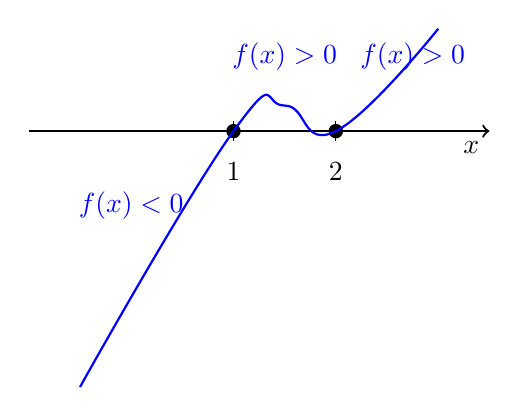
\begin{tikzpicture}[scale=1.3]
			\draw[->, thick] (-1,0) -- (3.5,0) node[below left] {$x$};
			
			\foreach \x/\label in {1/1, 2/2}{
				\draw (\x, 0.1) -- (\x, -0.1) node[below=4pt] {$\label$};
				\fill (\x,0) circle (2pt);
			}
			
			\draw[blue, thick] plot[smooth, tension=0.8] coordinates { (3, 1) (2,0) (1.5, 0.25) (1,0) (-0.5, -2.5) };
			
			\node[above, blue] at (2.75, 0.5) {$f(x)>0$};
			\node[above, blue] at (1.5, 0.5) {$f(x)>0$};
			\node[below, blue] at (0, -0.5) {$f(x)<0$};
			
		\end{tikzpicture}
		\caption{函数 $f(x)=(x-1)(x-2)^2$ 的图像示意}
	\end{figure}
	从上图可以清晰地看到,函数在 $x=2$ 点处触及x轴后并未穿过,形成了一个极小值点,符合题意.
	计算 $f(0)$:
	\begin{equation}
		f(0) = (0-1)(0-2)^2 = (-1)(4) = -4
	\end{equation}
	所以,最终答案是 -4.
\end{solution}
\qed


\subsection{含绝对值的不等式}

解含绝对值不等式的核心思想是“去掉绝对值符号”,主要有三种方法:

\begin{enumerate}
	\item \textbf{公式法}:利用基本模型 $|f(x)| < a \iff -a < f(x) < a$ 和 $|f(x)| > a \iff f(x) > a \text{ 或 } f(x) < -a$ (其中 $a>0$).
	\item \textbf{零点分段讨论法}:找到所有绝对值内部表达式的零点,用零点将数轴划分为若干区间,在每个区间上分别求解.
	\item \textbf{几何意义法}:利用 $|x-a|$ 表示数轴上点 $x$ 到点 $a$ 的距离.
\end{enumerate}

\begin{exercise}
	解不等式 $|x+1| - |x-2| \ge 1$.
\end{exercise}

\begin{solution}[零点分段法]
	零点为 $x=-1$ 和 $x=2$.它们将数轴分为三个区间,如图~\ref{fig:fenduan} 所示.
	
	\begin{itemize}
		\item \textbf{区间1 ($x < -1$)}:$-(x+1) + (x-2) \ge 1 \implies -3 \ge 1$.无解.
		\item \textbf{区间2 ($-1 \le x < 2$)}:$(x+1) + (x-2) \ge 1 \implies 2x-1 \ge 1 \implies x \ge 1$.取交集得 $1 \le x < 2$.
		\item \textbf{区间3 ($x \ge 2$)}:$(x+1) - (x-2) \ge 1 \implies 3 \ge 1$.恒成立.取交集得 $x \ge 2$.
	\end{itemize}
	综合所有区间的解,得到原不等式的解集为 $[1, \infty)$.
\end{solution}
\qed

\begin{figure}[H]
	\centering
	\begin{tikzpicture}[scale=1.2]
		% 坐标轴
		\draw[->, thick] (-3.5,0) -- (4.5,0) node[below left] {$x$};
		
		% 标出零点和分割线
		\foreach \x/\label in {-1/-1, 2/2}{
			\draw (\x, 0.2) -- (\x, -0.2) node[below=4pt] {$\label$};
			\draw[dashed] (\x, -0.5) -- (\x, 1.2);
		}
		
		% 标出区间名称
		\node[above] at (-2.25, 0.8) {区间1};
		\node[above] at (0.5, 0.8) {区间2};
		\node[above] at (3.25, 0.8) {区间3};
		
		% 标出最终解集
		\draw[line width=3pt, red] (1, -0.3) -- (4.5, -0.3);
		\fill[red] (1, -0.3) circle (2pt);
		\draw (1, -0.3) node[below=4pt, black] {$1$};
		\node[above, red] at (2.75, -0.3) {最终解集};
	\end{tikzpicture}
	\caption{零点分段法示意图}
\end{figure}

\section{柯西不等式}

如果说均值不等式是处理“和与积”问题的专家,那么柯西不等式则是一位处理“\textbf{平方和}”与“\textbf{和的平方}”之间关系的全能大师.它不受“正数”的限制(实数即可),形式灵活多变,威力巨大,在求最值、证不等式等领域都有着极其广泛的应用,被誉为“万能不等式”之一.掌握柯西不等式,将为你解决许多看似棘手的问题提供一个全新的、强有力的视角.


\subsection{柯西不等式的基本形式}

\begin{theorem}[柯西不等式二维形式]
	设 $a, b, x, y$ 均为实数,则:
	\begin{equation}
		\textcolor{red}{(a^2+b^2)(x^2+y^2) \ge (ax+by)^2}
	\end{equation}
	当且仅当 $\frac{a}{x} = \frac{b}{y}$ 时(或 $ay=bx$),等号成立.
\end{theorem}

\begin{theorem}[柯西不等式三维形式]
	设 $a, b, c, x, y, z$ 均为实数,则:
	\begin{equation}
		(a^2+b^2+c^2)(x^2+y^2+z^2) \ge (ax+by+cz)^2
	\end{equation}
	当且仅当 $\frac{a}{x} = \frac{b}{y} = \frac{c}{z}$ 时,等号成立.
\end{theorem}

\begin{note}
	该不等式可以推广到任意n维形式.在高中阶段,我们主要掌握其二维和三维形式的应用.其核心结构是:\textbf{(一堆数的平方和)乘以(另一堆数的平方和)大于等于(对应数乘积之和)的平方.}
\end{note}

\subsection{向量法证明}

\textcolor{green!50!black}{柯西不等式的结构与向量的坐标运算形式高度相似,这启发我们使用向量工具来证明它.向量法不仅形式上最为优美,也最能揭示不等式成立的几何本质.}

\begin{proof}[二维形式的向量证明]
		在平面直角坐标系中,我们构造两个向量:
		$\vec{m} = (a, b)$
		$\vec{n} = (x, y)$
		\begin{itemize}
			\item 代数表示:$\vec{m} \cdot \vec{n} = ax+by$
			\item 几何表示:$\vec{m} \cdot \vec{n} = |\vec{m}||\vec{n}|\cos\theta$,其中 $\theta$ 是两向量的夹角.
			\begin{figure}[H]
				\centering
				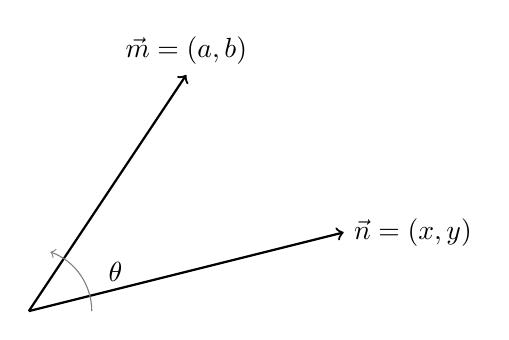
\begin{tikzpicture}
					\draw[->, thick] (0,0) -- (4,1) node[right] {$\vec{n}=(x,y)$};
					\draw[->, thick] (0,0) -- (2,3) node[above] {$\vec{m}=(a,b)$};
					\draw[->, gray] (0.8,0) arc (0:70:0.8);
					\node at (1.1, 0.5) {$\theta$};
				\end{tikzpicture}
				\caption{向量夹角示意图}
			\end{figure}
		\end{itemize}
		
		由数量积的两种表示相等,我们有:
		$ax+by = |\vec{m}||\vec{n}|\cos\theta$
		将两边同时平方,得到:
		$(ax+by)^2 = (|\vec{m}||\vec{n}|\cos\theta)^2 = |\vec{m}|^2 |\vec{n}|^2 \cos^2\theta$

		因为 $\cos^2\theta \le 1$,所以:
		$|\vec{m}|^2 |\vec{n}|^2 \cos^2\theta \le |\vec{m}|^2 |\vec{n}|^2$
		即 $(ax+by)^2 \le |\vec{m}|^2 |\vec{n}|^2$

		我们知道 $|\vec{m}|^2 = a^2+b^2$,$|\vec{n}|^2 = x^2+y^2$.
		代入上式,即得:
		$(ax+by)^2 \le (a^2+b^2)(x^2+y^2)$
		
		等号成立的条件是 $\cos^2\theta = 1$,这意味着 $\cos\theta = \pm 1$,即 $\theta=0$ 或 $\theta=\pi$.
		从几何上看,这意味着向量 $\vec{m}$ 与 $\vec{n}$ \textbf{共线}.
		从代数上看,共线意味着存在实数 $k$,使得 $\vec{m} = k\vec{n}$,即 $(a,b)=k(x,y)$.
		所以 $a=kx, b=ky$.当 $x,y$ 不为零时,即 $\frac{a}{x}=\frac{b}{y}=k$.
	三维形式的证明完全同理,只需构造三维向量 $\vec{m}=(a,b,c)$ 和 $\vec{n}=(x,y,z)$ 即可.
\end{proof}
\qed

\subsection{柯西不等式的信号与常见用法}

\textbf{【核心技巧】}
\textcolor{green!50!black}{如何判断一道题可能需要用到柯西不等式?关键是识别出题目中存在的“\textbf{平方和}”与“\textbf{一次式}”的结构.}
\begin{itemize}
	\item \textbf{信号一:题目条件或结论中出现 $x^2+y^2$ 或 $a^2+b^2+c^2$ 这样的平方和形式.}
	\item \textbf{信号二:题目条件或结论中出现 $ax+by$ 或 $ax+by+cz$ 这样的一次齐次式.}
\end{itemize}
柯西不等式的本质作用,就是建立起了这两种结构之间的桥梁:$(a^2+b^2)(x^2+y^2) \ge (ax+by)^2$.

\subsubsection{用法一:求最值}
这是柯西不等式在高考中最常见的应用.

\begin{exercise}
	已知实数 $x,y$ 满足 $3x+4y=10$,求 $x^2+y^2$ 的最小值.
\end{exercise}
\begin{solution}
	\textbf{【思路分析】}
	\textcolor{green!50!black}{我们观察到,条件是“一次式” ($3x+4y$),结论是求“平方和” ($x^2+y^2$) 的最值.这完美匹配了柯西不等式的结构.}
	
	\textbf{【解题步骤】}
	\begin{enumerate}
		\item \textbf{识别并构造不等式}:
		将 $3x+4y$ 看作 $ax+by$ 的形式,其中 $a=3, b=4$.
		将 $x^2+y^2$ 看作 $x^2+y^2$ 的形式.
		直接套用柯西不等式二维形式:
		$(a^2+b^2)(x^2+y^2) \ge (ax+by)^2$
		
		\item \textbf{代入已知量}:
		$(3^2+4^2)(x^2+y^2) \ge (3x+4y)^2$
		$25(x^2+y^2) \ge (10)^2$
		$25(x^2+y^2) \ge 100$
		
		\item \textbf{求解最值}:
		$x^2+y^2 \ge 4$
		所以 $x^2+y^2$ 的最小值为4.
		
		\item \textbf{【易错陷阱】检验等号能否取到}:
		\textcolor{red}{任何用不等式求出的最值,都必须验证其等号成立的条件能否满足,否则只是一个界,不一定是最值.}
		柯西不等式取等的条件是 $\frac{x}{a} = \frac{y}{b}$,在本题中即 $\frac{x}{3} = \frac{y}{4}$.
		设 $\frac{x}{3} = \frac{y}{4} = k$,则 $x=3k, y=4k$.
		将此代入约束条件 $3x+4y=10$ 中:
		$3(3k) + 4(4k) = 10 \implies 9k+16k=10 \implies 25k=10 \implies k=\frac{2}{5}$.
		此时,$x=3k=\frac{6}{5}, y=4k=\frac{8}{5}$.
		因为能找到具体的 $x,y$ 使等号成立,所以最小值确实是4.
	\end{enumerate}
	\textbf{【最终答案】} $x^2+y^2$ 的最小值为 $\textcolor{red}{4}$.
\end{solution}
\qed

\subsubsection{用法二:证明不等式}
柯西不等式是证明某些特定结构不等式的利器.

\begin{exercise}
	已知 $a,b,c$ 均为正数,求证:$(a+b+c)(\frac{1}{a}+\frac{1}{b}+\frac{1}{c}) \ge 9$.
\end{exercise}
\begin{solution}
	\textbf{【思路分析】}
	\textcolor{green!50!black}{这个不等式虽然可以用均值不等式证明,但用柯西不等式会更加直接.关键在于如何看出柯西不等式的结构.我们可以通过“开方配凑”的方法.}
	
	\textbf{【解题步骤】}
	\begin{enumerate}
		\item \textbf{构造平方和}:
		将 $a+b+c$ 看作 $(\sqrt{a})^2 + (\sqrt{b})^2 + (\sqrt{c})^2$.
		将 $\frac{1}{a}+\frac{1}{b}+\frac{1}{c}$ 看作 $(\frac{1}{\sqrt{a}})^2 + (\frac{1}{\sqrt{b}})^2 + (\frac{1}{\sqrt{c}})^2$.
		
		\item \textbf{套用三维柯西不等式}:
		设 $x_1=\sqrt{a}, x_2=\sqrt{b}, x_3=\sqrt{c}$
		设 $y_1=\frac{1}{\sqrt{a}}, y_2=\frac{1}{\sqrt{b}}, y_3=\frac{1}{\sqrt{c}}$
		
		$(x_1^2+x_2^2+x_3^2)(y_1^2+y_2^2+y_3^2) \ge (x_1y_1+x_2y_2+x_3y_3)^2$
		
		\item \textbf{代入并计算}:
		左边即为 $(a+b+c)(\frac{1}{a}+\frac{1}{b}+\frac{1}{c})$.
		右边为 $(\sqrt{a}\cdot\frac{1}{\sqrt{a}} + \sqrt{b}\cdot\frac{1}{\sqrt{b}} + \sqrt{c}\cdot\frac{1}{\sqrt{c}})^2$
		$= (1+1+1)^2 = 3^2 = 9$.
		
		\item \textbf{得出结论}:
		所以 $(a+b+c)(\frac{1}{a}+\frac{1}{b}+\frac{1}{c}) \ge 9$.
		当且仅当 $\frac{\sqrt{a}}{1/\sqrt{a}} = \frac{\sqrt{b}}{1/\sqrt{b}} = \frac{\sqrt{c}}{1/\sqrt{c}}$,即 $a=b=c$ 时,等号成立.原命题得证.
	\end{enumerate}
\end{solution}
\qed


\section{不等式恒成立问题}

有一类问题,它们不追求一个精确的解,而是探寻一种永远成立的条件.这就是\textbf{不等式恒成立问题}.它通常表现为:给定一个含有变量 $x$ 和参数 $a$ 的不等式,要求我们找到参数 $a$ 的取值范围,使得这个不等式对于指定范围内\textbf{所有}的 $x$ 都成立.这类问题是函数、方程与不等式知识的集大成者,深刻体现了存在与任意、特殊与一般的辩证观,是高考数学的核心热点与难点之一.


\begin{theorem}[恒成立问题的核心转化思想]
	不等式恒成立问题,其本质是\textbf{函数最值}问题.关键在于将“对于任意 $x$”的逻辑语言,转化为“函数的最值”的代数语言.
	\begin{itemize}
		\item 使不等式 $f(x) \le a$ 对任意 $x \in D$ 恒成立 $\iff$ \textcolor{red}{$a \ge f(x)_{\text{max}}$} 在区间 $D$ 上.
		\item 使不等式 $f(x) \ge a$ 对任意 $x \in D$ 恒成立 $\iff$ \textcolor{red}{$a \le f(x)_{\text{min}}$} 在区间 $D$ 上.
	\end{itemize}
	\textbf{【记忆口诀】} \textcolor{blue}{要让参数 $a$ 永远比一个函数大,就必须让 $a$ 大于等于这个函数的“天花板”(最大值);要让 $a$ 永远比一个函数小,就必须让 $a$ 小于等于这个函数的“地板”(最小值).简记为:“\textbf{大要大于等于最大,小要小于等于最小}”.}
\end{theorem}

\subsection{法一:参数分离法}

\begin{definition}[参数分离法]
	当不等式中的参数可以被代数式轻松地分离到不等号的一侧时,我们优先考虑使用此方法.它将原问题直接转化为我们最熟悉的求函数最值问题,思路清晰,步骤明确,是解决恒成立问题的首选策略.
\end{definition}

\begin{note}[核心步骤]
	\begin{enumerate}
		\item \textbf{分离参数}: 通过恒等变形,将参数移到不等式的一边,含变量 $x$ 的表达式移到另一边,得到 $a \ge g(x)$ 或 $a \le g(x)$ 的形式.
		\item \textbf{构造函数}: 构造新函数,即 $g(x)$.
		\item \textbf{求其最值}: 利用导数、基本不等式、函数单调性等工具,求出 $g(x)$ 在给定定义域内的最大值或最小值.
		\item \textbf{得出范围}: 根据核心转化思想,写出参数 $a$ 的取值范围.
	\end{enumerate}
\end{note}

\begin{exercise}
	若不等式 $x^2 + \frac{a}{x} \ge 1$ 对任意 $x \in [1, 2]$ 恒成立,求实数 $a$ 的取值范围.
\end{exercise}
\begin{solution}
	\textcolor{green!50!black}{观察不等式结构,参数 $a$ 仅出现在 $\frac{a}{x}$ 这一项中,很容易通过代数变形将其单独分离出来.因此,我们果断选择参数分离法.}

		$x^2 + \frac{a}{x} \ge 1 \implies \frac{a}{x} \ge 1 - x^2$.
		\textcolor{red}{【易错陷阱!】此时需要将分母的 $x$ 乘到不等式右边.进行这一步操作前,必须严格检查 $x$ 的正负!因为乘以负数会导致不等号反向.}
		\textcolor{blue}{在本题中,已知 $x \in [1, 2]$,显然 $x$ 是正数,所以我们可以放心地将 $x$ 乘到右边,且\textbf{不等号方向不变}.}
		$a \ge x(1-x^2) = x - x^3$.

		令 $g(x) = x - x^3$,其定义域为 $x \in [1, 2]$.
		根据核心转化思想,原问题转化为求 $a \ge g(x)_{\max}$ 在区间 $[1, 2]$ 上的值.
		
		\textcolor{blue}{【核心技巧】研究复杂函数(如三次及以上多项式)的单调性,求导是我们的首选武器.}
		对 $g(x)$ 求导,得 $g'(x) = 1 - 3x^2$.
		当 $x \in [1, 2]$ 时,$x^2 \in [1, 4]$,所以 $3x^2 \in [3, 12]$.
		因此,导数 $g'(x) = 1 - 3x^2 \le 1 - 3 = -2 < 0$.
		\textcolor{blue}{导数恒为负,说明函数 $g(x)$ 在整个区间 $[1, 2]$ 上是\textbf{严格单调递减}的.}

		对于单调递减的函数,其最大值在区间的\textbf{左端点}取得.
		$g(x)_{\max} = g(1) = 1 - 1^3 = 0$.
		根据“大要大于等于最大”的原则,我们必须有 $a \ge g(x)_{\max} = 0$.
	\textbf{【最终答案】} 实数 $a$ 的取值范围是 $\textcolor{red}{[0, +\infty)}$.
\end{solution}
\qed

\subsection{法二:函数最值法(分类讨论)}

\begin{definition}[函数最值法]
	当参数与变量纠缠在一起,难以分离(或分离后得到的新函数求最值非常困难)时,我们就放弃分离.直接将整个不等式看作一个关于 $x$ 的新函数(其中含有参数 $a$),通过讨论这个新函数的性质(尤其是最值)来解决问题.
\end{definition}

\begin{exercise}
	若不等式 $x^2 - 2ax + a > 0$ 对任意 $x \in [1, +\infty)$ 恒成立,求实数 $a$ 的取值范围.
\end{exercise}
\begin{solution}
	\textcolor{green!50!black}{参数 $a$ 同时出现在一次项和常数项,强行分离参数会得到 $a < \frac{x^2}{2x-1}$ (需讨论 $2x-1$ 的正负),右侧函数求最值较为繁琐.因此,我们转而构造一个关于x的二次函数,通过研究其最小值来求解.}
	
	令 $f(x) = x^2 - 2ax + a$.问题转化为求 $f(x)_{\min} > 0$ 在区间 $[1, +\infty)$ 上恒成立.
	\textcolor{blue}{【核心技巧】这是一个开口向上的二次函数,其性质完全由\textbf{对称轴} $x = -\frac{-2a}{2 \cdot 1} = a$ 的位置决定.解决这类问题的灵魂,就在于讨论“对称轴”与“给定区间”的相对位置.}
	
	\begin{figure}[H]
		\centering
		\begin{tikzpicture}[scale=1]

			\begin{scope}
				\node at (1.5, 3.5) {情况一: $a < 1$ (对称轴在区间左侧)};
				\draw[->] (-1,0) -- (4,0) node[below] {$x$};
				\draw[thick, gray, pattern=north east lines] (1,0) rectangle (4, 0.2);
				\node[above] at (2.5,0.2) {定义域 $[1, \infty)$};
				\draw[blue, thick, smooth, domain=-0.5:3.5] plot (\x, {(\x-0.5)^2+1});
				\draw[red, dashed] (0.5, 0) node[below, black]{$a$}-- (0.5, 3);
				\node[above, red] at (0.5,3) {对称轴};
				\fill[red] (1, 1.25) circle (2pt) node[right,black]{$f(1)$是最小值};
			\end{scope}

			\begin{scope}[xshift=7cm]
				\node at (1.5, 3.5) {情况二: $a \ge 1$ (对称轴在区间内)};
				\draw[->] (-1,0) -- (4,0) node[below] {$x$};
				\draw[thick, gray, pattern=north east lines] (1,0) rectangle (4, 0.2);
				\node[above] at (2.5,0.2) {定义域 $[1, \infty)$};
				\draw[blue, thick, smooth, domain=-0.5:3.5] plot (\x, {(\x-2)^2+1});
				\draw[red, dashed] (2, 0) node[below, black]{$a$}-- (2, 3);
				\node[above, red] at (2,3) {对称轴};
				\fill[red] (2, 1) circle (2pt) node[below left,black]{$f(a)$是最小值};
			\end{scope}
		\end{tikzpicture}
		\caption{二次函数对称轴与区间的关系}
	\end{figure}
	
	\textbf{【解题步骤】}
	\begin{enumerate}
		\item \textbf{情况一:对称轴在区间左侧 ($a < 1$)}
		\textcolor{blue}{此时,函数 $f(x)$ 在区间 $[1, +\infty)$ 上是\textbf{单调递增}的.其“地板”(最小值)就在区间的入口处取得.}
		最小值为:$f(x)_{\min} = f(1) = 1^2 - 2a(1) + a = 1-a$.
		我们需要 $f(x)_{\min} > 0$,即 $1-a > 0 \implies a < 1$.
		\textcolor{blue}{将此结论与本情况的大前提 $a < 1$ 取交集,结果仍为 $\textcolor{blue}{a < 1}$.}
		
		\item \textbf{情况二:对称轴在区间内部或与之重合 ($a \ge 1$)}
		\textcolor{blue}{此时,函数 $f(x)$ 的“地板”(最小值)就在抛物线的顶点处取得.}
		其最小值为:$f(x)_{\min} = f(a) = a^2 - 2a(a) + a = -a^2+a$.
		我们需要 $f(x)_{\min} > 0$,即 $-a^2+a > 0 \implies a^2-a < 0 \implies a(a-1) < 0$.
		解得 $0 < a < 1$.
		\textcolor{red}{将此结论与本情况的大前提 $a \ge 1$ \textbf{取交集},发现没有任何公共部分,所以此种情况无解,解集为 $\textcolor{blue}{\emptyset}$.}
		
		\item \textbf{综合结论}:
		将两种情况的解集取并集:$(-\infty, 1) \cup \emptyset$.
	\end{enumerate}
	实数 $a$ 的取值范围是 $\textcolor{red}{(-\infty, 1)}$.
\end{solution}
\qed

\subsection{法三:数形结合法}

\begin{definition}[数形结合法]
	将不等式两边看作两个函数的图像,恒成立问题就转化为一个函数的图像恒在另一个函数图像的上方(或下方)的问题.这种方法能将抽象的代数问题转化为直观的几何问题,尤其适用于那些两边函数图像易于绘制的情形.
\end{definition}

\begin{exercise}
	若不等式 $\sqrt{x} \ge ax$ 对任意 $x \ge 0$ 恒成立,求实数 $a$ 的取值范围.
\end{exercise}
\begin{solution}
	\textcolor{green!50!black}{不等式的一边是 $y_1 = \sqrt{x}$,它的图像我们非常熟悉;另一边是 $y_2 = ax$,它表示一条过原点、斜率为 $a$ 的直线.问题可以直观地翻译为:在 $y$ 轴右侧(包括 $y$ 轴),曲线 $y_1 = \sqrt{x}$ 必须始终在直线 $y_2=ax$ 的上方或者与它相交.}


		精确地画出 $y_1 = \sqrt{x}$ 的图像.它是一个过原点,在第一象限单调递增的“半个”抛物线.
		
		直线 $y_2 = ax$ 是一个绕着原点 $(0,0)$ 旋转的“动态”图像.我们根据斜率 $a$ 的正负来讨论.
		
		\begin{figure}[H]
			\centering
			\begin{tikzpicture}[scale=1.2]
				\draw[->] (-1,0) -- (5,0) node[below] {$x$};
				\draw[->] (0,-2) -- (0,3) node[left] {$y$};
				\node[below left] at (0,0) {$O$};
				
				\draw[blue, very thick, domain=0:4.5, samples=100] plot (\x, {sqrt(\x)}) node[above] {$y_1=\sqrt{x}$};
				
				\draw[red, thick, dashed] (0,0) -- (2, 2.5) node[right] {$a>0$ (不满足)};
				\node at (1.5, 1.22) {$\times$};
				\node[below, red] at (1.5, 1.22) {直线在上};

				\draw[purple, thick] (-1,0) -- (4.5,0) node[above right] {$a=0$ (满足)};

				\draw[purple, thick] (0,0) -- (4, -1.6) node[below right] {$a<0$ (满足)};
			\end{tikzpicture}
			\caption{$y_1=\sqrt{x}$ 与不同斜率的直线 $y_2=ax$ 的位置关系}
		\end{figure}
		
		\begin{itemize}
			\item \textbf{\textcolor{blue}{情况一:当 $a > 0$ 时}}
			\textcolor{blue}{此时直线在第一象限.从图像可以看出,虽然直线在原点附近会被曲线“压在身下”,但由于直线是“笔直”上升的,而曲线的增长越来越“平缓”,所以直线最终总会“穿过”并跑到曲线的上方去.}
			\textcolor{red}{因此,只要 $a>0$,就不可能满足对“所有”$x\ge 0$ 都成立的要求.此种情况无解.}
			
			\item \textbf{\textcolor{blue}{情况二:当 $a \le 0$ 时}}
			\textcolor{blue}{若 $a=0$,直线为 $y=0$ (x轴).$\sqrt{x} \ge 0$ 显然对所有 $x \ge 0$ 恒成立.}
			\textcolor{blue}{若 $a<0$,直线在第四象限.对于任意 $x>0$,我们有 $\sqrt{x} > 0$,而 $ax < 0$.一个正数永远大于一个负数.在 $x=0$ 时,$\sqrt{0}=a \cdot 0$,等号成立.}
			\textcolor{blue}{所以,当 $a \le 0$ 时,不等式 $\sqrt{x} \ge ax$ 恒成立.}
		\end{itemize}

		实数 $a$ 的取值范围是 $\textcolor{red}{(-\infty, 0]}$.
\end{solution}
\qed

\section{三角换元}

三角换元法的本质,是一种“\textbf{以曲代直}”的降维打击.它利用三角函数与生俱来的与圆的特殊关系,将一个复杂的、带有根号或平方和的\textbf{代数问题},巧妙地“翻译”成一个我们更擅长处理的、关于角度的\textbf{三角函数最值问题}.这不仅仅是一种计算技巧,更是一种深刻的数学思想——数形结合的极致体现.

\subsection{原理}

\textcolor{green!50!black}{三角换元法得以成立的理论基石,是三角函数中最基本、也最根本的恒等式——\textbf{同角三角函数关系}.}
\begin{itemize}
	\item \textbf{平方关系}: $\sin^2\theta + \cos^2\theta = 1$
	\item \textbf{商数关系}: $\tan\theta = \frac{\sin\theta}{\cos\theta}$
\end{itemize}
特别是平方关系,它完美地对应了代数中的“平方和”结构.

\textbf{【翻译过程揭秘】}
我们来看,这个“翻译”过程是如何发生的:
\begin{enumerate}
	\item \textbf{代数结构}: 考虑一个常见的代数结构 $\sqrt{R^2 - x^2}$,其中 $|x| \le R$.
	\item \textbf{引入换元}: 我们进行换元,令 $x = R\sin\theta$. 
	\textcolor{red}{【换元必换范围!】}既然 $|x| \le R$, 那么 $|R\sin\theta| \le R$, 即 $|\sin\theta| \le 1$. 我们可以自然地取 $\theta \in [-\frac{\pi}{2}, \frac{\pi}{2}]$, 在这个区间内,$\sin\theta$ 能取遍 $[-1,1]$ 中所有的值,且 $\cos\theta \ge 0$.
	\item \textbf{魔法开始了?}:
	\begin{align*}
		\sqrt{R^2 - x^2} &= \sqrt{R^2 - (R\sin\theta)^2} \\
		&= \sqrt{R^2 - R^2\sin^2\theta} \\
		&= \sqrt{R^2(1 - \sin^2\theta)} & \text{\textcolor{green!50!black}{(提公因式,创造核心结构)}} \\
		&= \sqrt{R^2\cos^2\theta} & \text{\textcolor{red}{(平方关系登场!)}} \\
		&= |R\cos\theta| \\
		&= R\cos\theta & \text{\textcolor{blue}{(因为我们选定 $\theta \in [-\frac{\pi}{2}, \frac{\pi}{2}]$, 所以 $\cos\theta \ge 0$)}}
	\end{align*}
\end{enumerate}
\textcolor{green!50!black}{看!通过三角换元,我们成功地将一个复杂的\textbf{无理式}(根式)“翻译”成了一个简洁的\textbf{三角式},彻底消灭了根号.这就是三角换元法的威力所在.}

\begin{note}[何时用三角换元?]
	当你看到以下这些结构时,就应该立刻对三角换元法保持高度警觉:
	\begin{itemize}
		\item \textbf{约束条件为圆或椭圆}: 变量 $x, y$ 满足 $x^2+y^2=R^2$ 或 $\frac{x^2}{a^2}+\frac{y^2}{b^2}=1$.
		\item \textbf{表达式中含特定根式}: 形如 $\sqrt{R^2-x^2}$ 的结构.
		\item \textbf{代数问题具有几何背景}: 问题可以抽象为求圆上或椭圆上的点到某直线距离的最值、或某个与坐标相关的表达式的最值.
	\end{itemize}
\end{note}

\subsection{运用指南}
\begin{enumerate}
	\item \textbf{识别信号,确定换元形式}:
	\begin{itemize}
		\item 若有 $x^2+y^2=R^2$, 可设 $\begin{cases} x = R\cos\theta \\ y = R\sin\theta \end{cases}$.
		\item 若有 $\frac{x^2}{a^2}+\frac{y^2}{b^2}=1$, 可设 $\begin{cases} x = a\cos\theta \\ y = b\sin\theta \end{cases}$.
		\item 若有 $\sqrt{R^2-x^2}$, 可设 $x = R\sin\theta$ 或 $x=R\cos\theta$.
	\end{itemize}
	\item \textbf{【重中之重】确定新元 $\theta$ 的范围}:
	\textcolor{red}{这是三角换元中最关键、最容易出错的一步!必须根据原变量 $x,y$ 的范围,确定新变量 $\theta$ 的取值范围.} 如果原变量没有范围限制,通常默认 $\theta \in [0, 2\pi)$.
	\item \textbf{代入化简,转化为三角函数问题}:
	将换元后的表达式代入所求的式子中,利用三角恒等变换(如辅助角公式、和差化积、倍角公式等)进行化简.
	\item \textbf{在 $\theta$ 的新范围内求解最值}:
	结合三角函数的图像和性质,求出目标函数在 $\theta$ 的允许范围内的最大值或最小值.
\end{enumerate}

\subsection{典例剖析}
\begin{exercise}
	已知实数 $x, y$ 满足 $x^2+y^2=4$,求 $z = x+y$ 的取值范围.
\end{exercise}
\begin{solution}
	\textbf{【思路分析】}
	\textcolor{green!50!black}{约束条件 $x^2+y^2=4$ 是一个标准圆的方程(半径 $R=2$),这是使用三角换元最直接、最强烈的信号.我们可以将圆上的任意一点 $P(x,y)$ 用其对应的圆心角 $\theta$ 来表示.}
	
	\textbf{【解题步骤】}

		根据 $x^2+y^2=2^2$,我们设:
		$\begin{cases} x = 2\cos\theta \\ y = 2\sin\theta \end{cases}$
		
		题目对 $x,y$ 没有额外的范围限制,因此点 $(x,y)$ 可以取遍整个圆周.我们取 $\theta \in [0, 2\pi)$.
		
		将换元形式代入目标函数 $z = x+y$:
		$z = 2\cos\theta + 2\sin\theta = 2(\sin\theta + \cos\theta)$
		\textcolor{blue}{这是一个典型的 $a\sin x + b\cos x$ 形式,我们使用辅助角公式进行化简.}
		$z = 2 \cdot \sqrt{1^2+1^2} \sin(\theta + \frac{\pi}{4}) = 2\sqrt{2}\sin(\theta + \frac{\pi}{4})$

		因为 $\theta \in [0, 2\pi)$,所以 $\theta+\frac{\pi}{4} \in [\frac{\pi}{4}, \frac{9\pi}{4})$.
		这个新区间 $[\frac{\pi}{4}, \frac{9\pi}{4})$ 的长度为 $2\pi$,完整地覆盖了一个周期.
		因此,$\sin(\theta + \frac{\pi}{4})$ 可以取到其最大值 $1$ 和最小值 $-1$.
		
		\begin{itemize}
			\item 当 $\sin(\theta+\frac{\pi}{4}) = 1$ 时,$z$ 取得最大值 $z_{\max} = 2\sqrt{2} \times 1 = 2\sqrt{2}$.
			\item 当 $\sin(\theta+\frac{\pi}{4}) = -1$ 时,$z$ 取得最小值 $z_{\min} = 2\sqrt{2} \times (-1) = -2\sqrt{2}$.
		\end{itemize}
	
	\begin{figure}[H]
		\centering
		\begin{tikzpicture}[scale=1.2]
			\draw[->] (-3,0) -- (3,0) node[below] {$x$};
			\draw[->] (0,-3) -- (0,3) node[left] {$y$};
			\draw[thick, blue] (0,0) circle (2);
			\node[blue, right] at (2,0) {$x^2+y^2=4$};


			\draw[red, dashed] (-0.5, 3.328) -- (3.328, -0.5) node[right, black] {$y=-x+2\sqrt{2}$ (相切)};
			\fill[red] (1.414, 1.414) circle (1.5pt) node[above right] {$P_1$};

			\draw[red, dashed] (0.5, -3.328) -- (-3.328, 0.5) node[left, black] {$y=-x-2\sqrt{2}$ (相切)};
			\fill[red] (-1.414, -1.414) circle (1.5pt) node[below left] {$P_2$};
			\node at (2.5,-2.5) {\textbf{几何意义:} $z=x+y$ 的最值,就是直线族(即一组直线) $y=-x+z$ 的截距 $z$ 的最值.当直线与圆相切时,截距取得最值.};
		\end{tikzpicture}
		\caption{三角换元的几何直观}
	\end{figure}
	
	\textbf{【最终答案】} $z=x+y$ 的取值范围是 $\textcolor{red}{[-2\sqrt{2}, 2\sqrt{2}]}$.
\end{solution}
\qed

\section*{不等式章后总结}

\lettrine{恭}{喜你},完成了不等式这一篇章!从此刻起,你手中的数学解题工具箱又增添了几件削铁如泥的利器.不等式不仅是高考中的独立考点,更是贯穿于函数、数列、解析几何、立体几何等几乎所有高中数学分支的底层逻辑与核心工具.

本章的挑战,不在于记忆繁多的公式,而在于领悟“\textbf{转化}”与“\textbf{构造}”的艺术.无论是均值不等式中“\textbf{一正、二定、三相等}”的严苛戒律,还是柯西不等式在“\textbf{平方和}”与“\textbf{和的平方}”之间架起的优雅桥梁,其灵魂都在于如何通过巧妙的“\textbf{配凑}”,将一个看似陌生的表达式,转化为我们熟悉的、可以施展这些“神兵”的标准形态.

当你能够做到:看到分式就想到“\textbf{拆项}”或“\textbf{乘1代换}”,看到根式就想到“\textbf{平方}”或“\textbf{三角换元}”,看到“恒成立”就想到“\textbf{函数最值}”,那么,你就真正掌握了不等式的精髓.愿你在后续的复习中,能时常回顾这些思想,将它们内化为你的数学直觉.

\subsection*{知识体系梳理与核心经验总结}

\begin{note}[核心框架]
	不等式一章的学习,可以归纳为“\textbf{一个中心,两大支柱,三种思想}”.
	\begin{itemize}
		\item \textbf{一个中心}:求解最值问题.
		\item \textbf{两大支柱}:\textbf{均值不等式} 与 \textbf{柯西不等式}.
		\item \textbf{三种思想}:\textbf{配凑思想}、\textbf{函数与方程思想}、\textbf{转化与化归思想}.
	\end{itemize}
\end{note}

\subsubsection*{不等式解法回顾}
\begin{itemize}
	\item \textbf{一元二次不等式}:核心是“三步法”——(1)标准化(二次项系数为正);(2)求根(十字相乘或公式法);(3)结合图像写解集(“大于取两边,小于取中间”).
	\item \textbf{高次/分式不等式}:通用武器是“\textbf{数轴标根法}”.务必牢记“\textbf{奇穿偶不穿}”的穿线原则,并对分式不等式,要额外注意\textbf{分母不为零}.
	\item \textbf{绝对值不等式}:最稳妥的方法是“\textbf{零点分段讨论}”,将问题化整为零,逐一击破.对于简单形式,可利用几何意义(数轴上的距离)或公式法($|x|<a \Leftrightarrow -a<x<a$)快速求解.
\end{itemize}

\subsubsection*{两大核心不等式辨析}
\begin{enumerate}
	\item \textbf{均值不等式 ($a,b>0 \Rightarrow \frac{a+b}{2} \ge \sqrt{ab}$)}
	\begin{itemize}
		\item \textbf{使用信号}:表达式中出现“和”与“积”的结构,尤其是分式形式(如 $x+\frac{k}{x}$).
		\item \textbf{核心戒律}:\textcolor{red}{“一正、二定、三相等”}.
		\begin{itemize}
			\item \textbf{一正}:各项必须为正数.
			\item \textbf{二定}:求最小值时,和为定值;求最大值时,积为定值.这是所有“配凑”技巧的目标.
			\item \textbf{三相等}:必须能找到使各项取值相等的点,否则求出的只是一个界,而非最值.
		\end{itemize}
	\end{itemize}
	\item \textbf{柯西不等式 ($(a^2+b^2)(x^2+y^2) \ge (ax+by)^2$)}
	\begin{itemize}
		\item \textbf{使用信号}:条件或结论中同时出现“\textbf{平方和}”(如 $x^2+y^2$)与“\textbf{一次齐次式}”(如 $ax+by$)这两种结构.
		\item \textbf{核心优势}:对变量正负没有要求(实数即可),形式灵活,是连接“平方和”与“和的平方”的万能桥梁.
		\item \textbf{取等条件}:各项成比例,即 $\frac{a}{x}=\frac{b}{y}$.
	\end{itemize}
\end{enumerate}

\subsubsection*{三大解题思想与策略}
\begin{description}
	\item[配凑思想] 这是不等式应用中的“第一生产力”,是化“不定”为“定”的关键.
	\begin{itemize}
		\item \textbf{拆项/凑项}:如 $x+\frac{1}{x-1} = (x-1)+\frac{1}{x-1}+1$.
		\item \textbf{凑系数}:如为配平 $2x+\frac{1}{x}$,可将 $2x$ 拆为 $x+x$ 或将 $\frac{1}{x}$ 乘以2再除以2.
		\item \textbf{乘“1”代换}:已知 $ax+by=k$,求 $\frac{c}{x}+\frac{d}{y}$ 的最值,核心是利用 $(\frac{c}{x}+\frac{d}{y}) \cdot 1 = (\frac{c}{x}+\frac{d}{y}) \frac{ax+by}{k}$ 来“配平次数”,创造出常数项和倒数项.
		\item \textbf{整体代换}:如三角换元,将代数问题转化为几何或三角函数问题.
	\end{itemize}
	\item[函数与方程思想] 将不等式问题转化为函数问题,是解决复杂不等式(尤其是恒成立问题)的根本途径.
	\begin{itemize}
		\item \textbf{恒成立 $\iff$ 最值}:$f(x) \ge a$ 恒成立 $\iff f(x)_{\min} \ge a$.
		\item \textbf{构造函数,研究性质}:利用导数等工具研究函数的单调性、极值,从而找到最值.
		\item \textbf{数形结合}:将不等式两边看作两个函数的图像,其大小关系转化为图像的上下位置关系,直观求解.
	\end{itemize}
	\item[转化与化归思想] 这是数学解题的普适性思想.将陌生问题转化为熟悉问题,将复杂问题转化为简单问题.例如,将分式不等式转化为整式不等式,将无理不等式转化为有理不等式,将超越不等式(含 $\ln x, e^x$ 等)利用导数转化为代数不等式.
\end{description}